\section{\textbf{Hierarchical Joint--Disjoint Agency}}

The disjoint and joint AGI-Former architectures need not be deployed as mutually exclusive alternatives. They can be composed into a hierarchy in which the joint-output architecture performs global coordination and disjoint-output architectures perform regional or specialized execution. In this organization, the global model generates unified supervisory action tokens that express a shared plan, while each regional model translates that plan into actions valid for its local observations, capabilities, and constraints.

Figure~\ref{fig:hierarchical_agi_former} illustrates the resulting recurrent control loop. Regional agents receive local multimodal observations and return state representations, action proposals, uncertainty estimates, and execution feedback. The global joint coordinator fuses this information and produces supervisory tokens encoding goals, priorities, constraints, or a coordinated plan. Those tokens condition the regional agents, which produce locally executable actions. Environmental consequences then generate new observations and feedback for the next cycle.

\begin{figure*}[t]
    \centering
    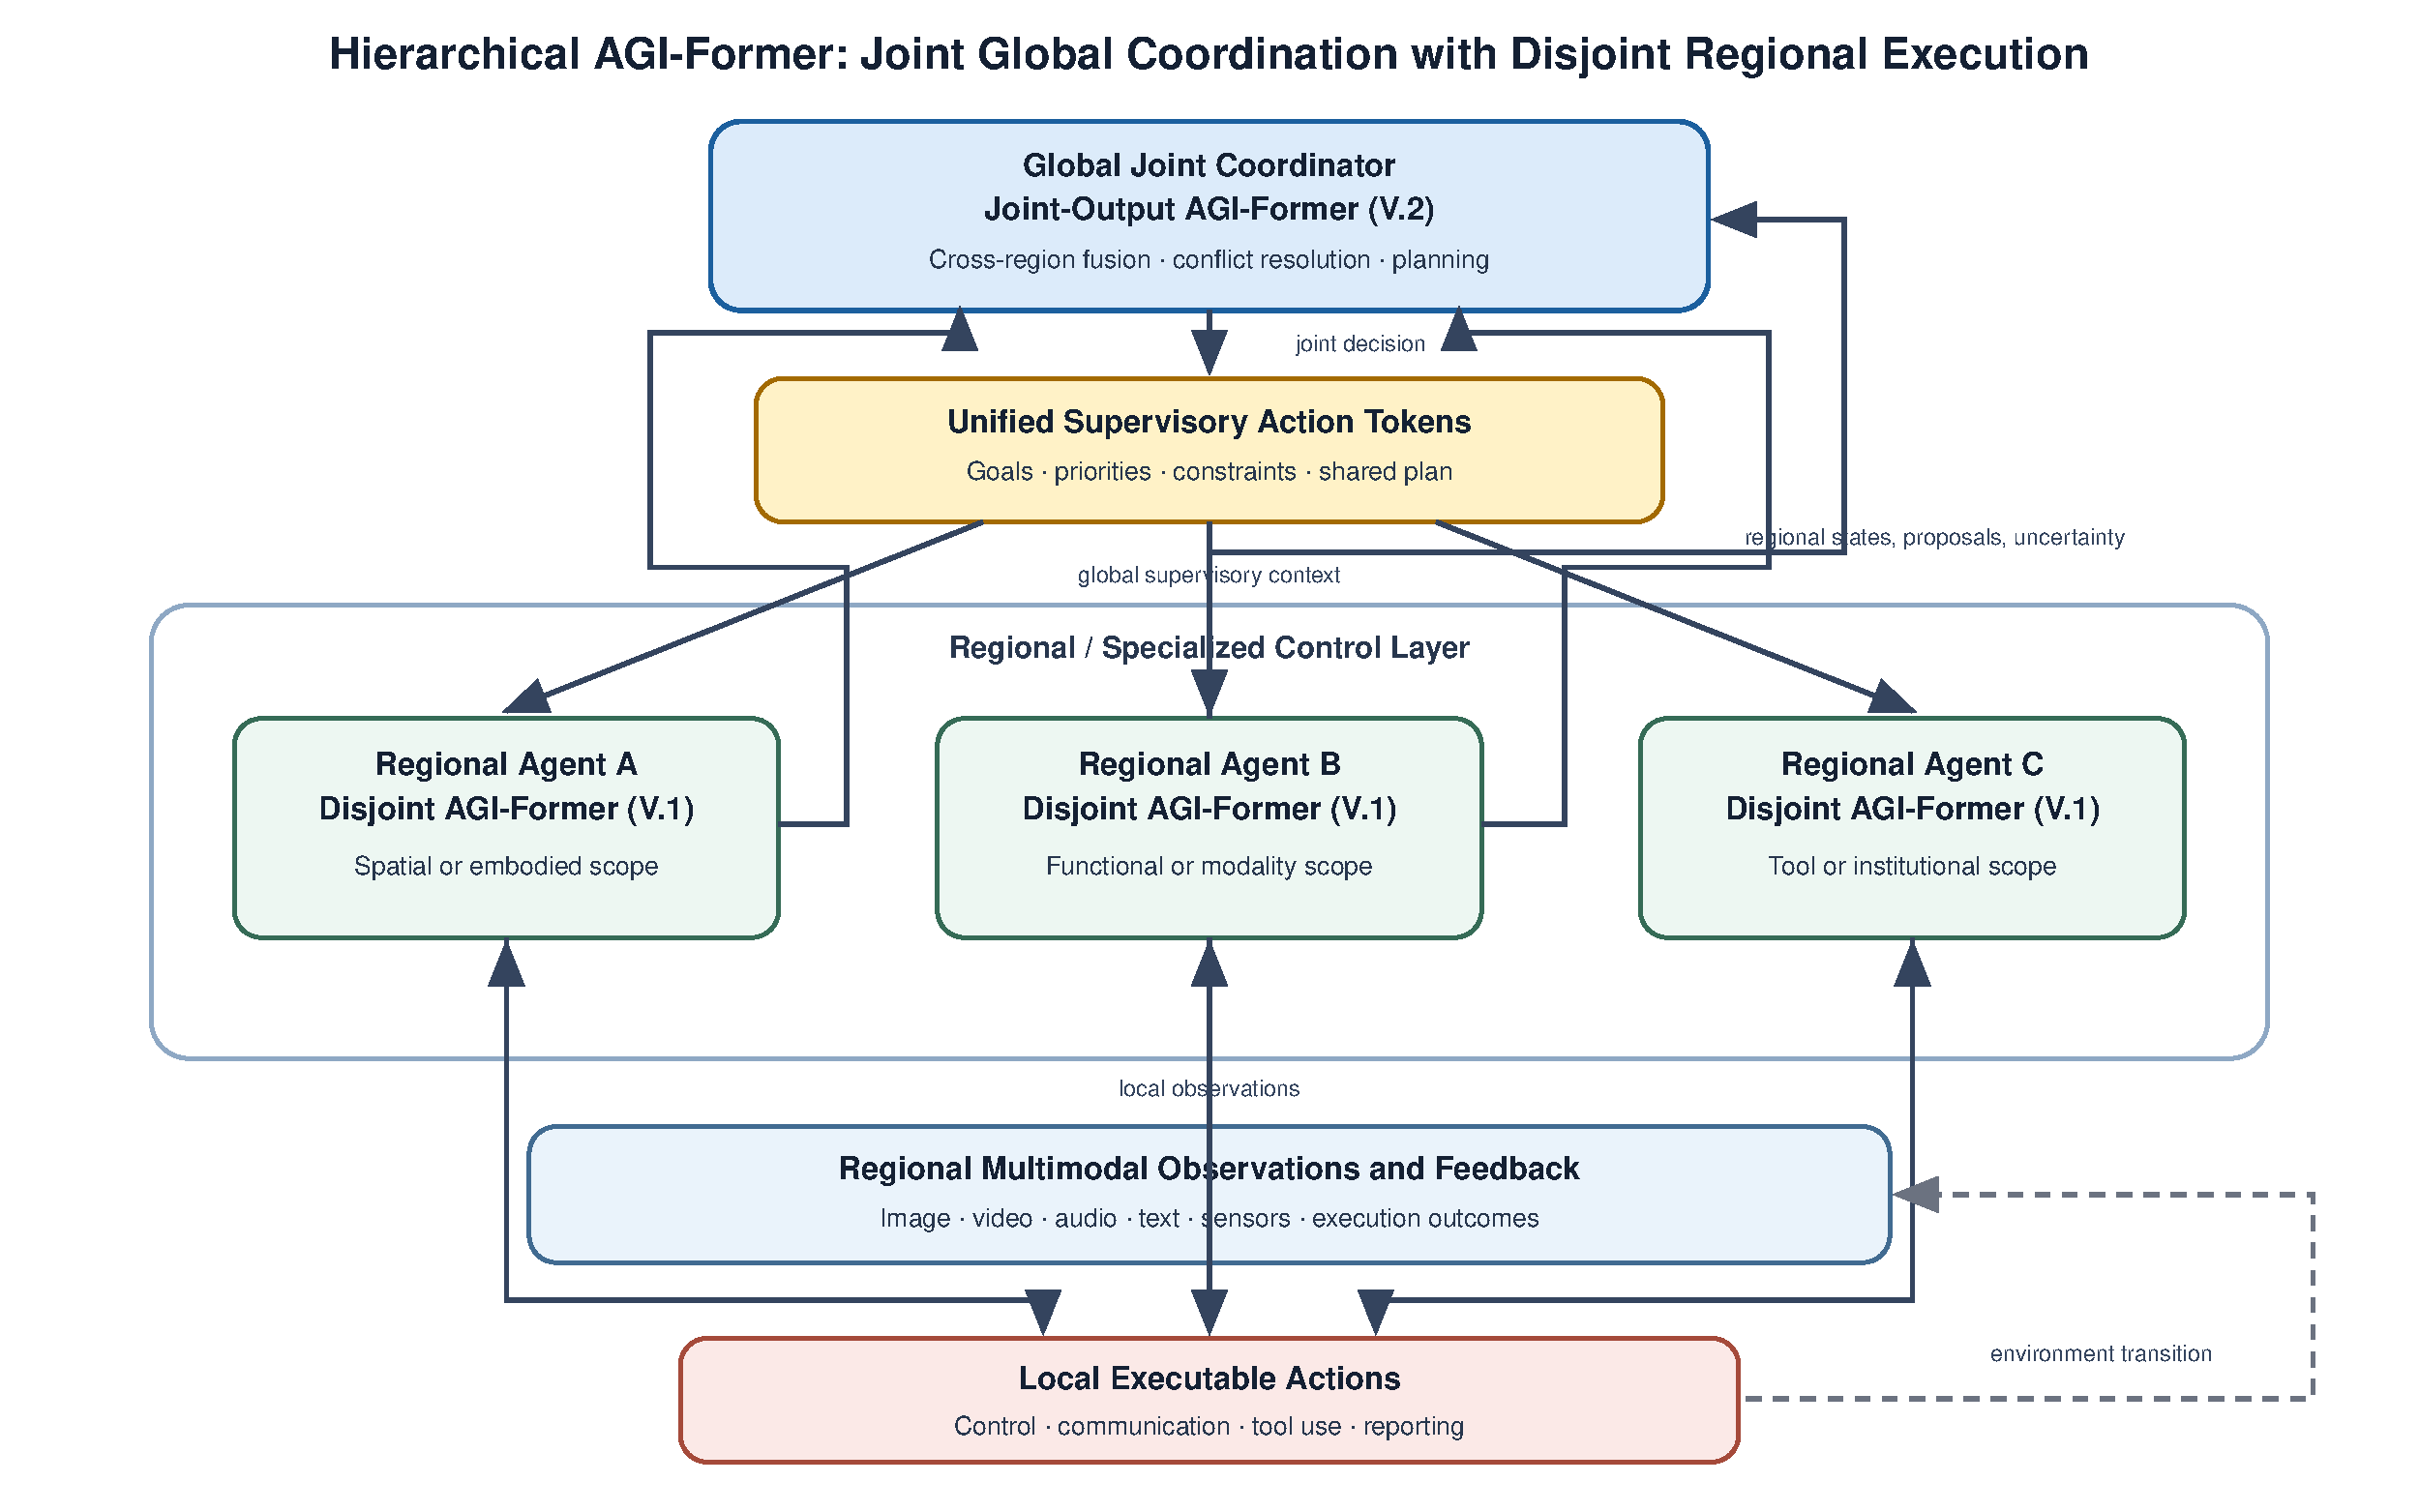
\includegraphics[width=\textwidth]{Figures/fig4.pdf}
    \caption{Hierarchical AGI-Former with joint global coordination and disjoint regional execution. Regional AGI-Former agents transform local observations and global supervisory context into specialized actions. Their states, proposals, uncertainty, and execution feedback are aggregated by a joint-output AGI-Former, which generates the supervisory tokens for the next control cycle.}
    \label{fig:hierarchical_agi_former}
\end{figure*}

\subsection{\textbf{Regional Agents and Scope}}

Let $\mathcal{R}=\{1,\ldots,R\}$ denote a set of regional agents. A region need not be geographic. It may correspond to a physical zone, robot, actuator group, modality, functional capability, software tool, institution, or administrative jurisdiction. Agent $r$ receives a local modality set $\mathcal{M}_r$ and maintains a local causal history $Y_{<t}^{(r)}$. Its encoded local context is

\begin{equation}
\begin{aligned}
    \mathcal{H}_t^{(r)}
    &= \left\{
       E_m^{(r)}\!\left(X_t^{(r,m)}\right):
       m\in\mathcal{M}_r,\;r_t^{(r,m)}=1
       \right\},\\
    S_t^{(r)}
    &= \operatorname{UMHAED}^{(r)}\!\left(
       Y_{<t}^{(r)}
       \right).
\end{aligned}
\label{eq:regional_context}
\end{equation}

Each regional agent is therefore an instance of the disjoint architecture, but its branches and output spaces may differ from those of other regions. A drone region may produce navigation and camera-control tokens, while a communication region may produce language and network-action tokens.

Let $s_r$ be a learned or structured scope token identifying the authority and capabilities of region $r$. Scope is included in both upward and downward communication so that identical token values cannot silently acquire different operational meanings across agents.

\subsection{\textbf{Upward Regional State and Proposal Tokens}}

Before the global decision, each regional agent compresses its current context into a bounded upward message:

\begin{equation}
\begin{aligned}
    q_t^{(r)}
    &= \operatorname{RegionalReadout}_{r}\!\left(
       S_t^{(r)},\mathcal{H}_t^{(r)},s_r
       \right),\\
    q_t^{(r)}
    &= \left[
       q_{t,\mathrm{state}}^{(r)};
       q_{t,\mathrm{proposal}}^{(r)};
       q_{t,\mathrm{uncertainty}}^{(r)};
       q_{t,\mathrm{feedback}}^{(r)}
       \right].
\end{aligned}
\label{eq:regional_upward_message}
\end{equation}

The four fields are logical token types rather than mandatory fixed-length vectors. State tokens describe locally relevant conditions; proposal tokens express candidate actions or requested resources; uncertainty tokens communicate confidence, missing information, or conflict; and feedback tokens summarize the outcome of previously executed commands.

The active regional messages form the global input memory

\begin{equation}
\begin{aligned}
    Q_t
    &= \mathop{\operatorname{Concat}}_{r\in\mathcal{R}_t}
       \left(q_t^{(r)}+e_r\right),\\
    \mathcal{R}_t
    &= \left\{r\in\mathcal{R}:a_t^{(r)}=1\right\},
\end{aligned}
\label{eq:global_regional_memory}
\end{equation}

where $e_r$ identifies the source region and $a_t^{(r)}$ indicates its availability. Regional dropout during training can vary $\mathcal{R}_t$ so that global coordination does not depend on every agent being continuously reachable.

\subsection{\textbf{Global Joint Coordination}}

The global coordinator is an instance of the joint-output architecture. It conditions its global causal state $S_k^{G}$ on $Q_t$ and generates a unified supervisory sequence $u_k$:

\begin{equation}
\begin{aligned}
    J_k^{G}
    &= \operatorname{JointAGIFormer}\!\left(
       S_k^{G},Q_t;\theta_G
       \right),\\
    u_k
    &\sim p_{\theta_G}\!\left(
       u_k\mid S_k^{G},Q_t
       \right).
\end{aligned}
\label{eq:global_supervision}
\end{equation}

The supervisory sequence may contain a global objective, ordered subgoals, resource assignments, temporal constraints, prohibitions, escalation conditions, and region-addressed directives. It is a learned action-token sequence, not merely a natural-language summary.

To prevent every region from receiving every directive, let $A_k\in\{0,1\}^{R\times |u_k|}$ be an address and authorization mask. The supervisory context visible to region $r$ is

\begin{equation}
\begin{aligned}
    u_k^{(r)}
    &= \operatorname{Select}\!\left(
       u_k,A_k[r,:],s_r
       \right).
\end{aligned}
\label{eq:regional_supervision_mask}
\end{equation}

This mechanism distinguishes shared plan tokens from restricted commands and allows the hierarchy to represent different permissions, capabilities, or information boundaries.

\subsection{\textbf{Regional Execution Under Global Context}}

Each regional agent treats $u_k^{(r)}$ as an additional causal condition rather than as an executable command by itself. The regional action distribution is

\begin{equation}
\begin{aligned}
    y_t^{(r)}
    &\sim p_{\theta_r}\!\left(
       y_t^{(r)}
       \mid S_t^{(r)},
       \mathcal{H}_t^{(r)},
       u_k^{(r)},
       c_t^{(r)}
       \right),
\end{aligned}
\label{eq:regional_execution}
\end{equation}

where $c_t^{(r)}$ contains local physical, legal, resource, and safety constraints. The disjoint regional architecture can emit several specialized streams when a region controls multiple tools or effectors. Thus, one global sequence may generate many locally valid actions without requiring a universal low-level control vocabulary.

The environment transition and feedback loop are

\begin{equation}
\begin{aligned}
    e_{t+1}
    &\sim \mathcal{P}\!\left(
       e_{t+1}\mid e_t,
       \{y_t^{(r)}\}_{r\in\mathcal{R}_t}
       \right),\\
    f_{t+1}^{(r)}
    &= \operatorname{FeedbackEnc}_{r}\!\left(
       x_{t+1}^{(r)},y_t^{(r)},c_{t+1}^{(r)}
       \right),\\
    q_{t+1,\mathrm{feedback}}^{(r)}
    &\leftarrow f_{t+1}^{(r)}.
\end{aligned}
\label{eq:hierarchical_feedback}
\end{equation}

The next global decision therefore depends on observed consequences, not solely on whether regional agents accepted the previous plan.

\subsection{\textbf{Multiple Control Time Scales}}

Global coordination and regional execution need not occur at the same frequency. Let $k$ index global planning intervals and let $t\in[b_k,b_{k+1})$ index local decisions governed by supervisory sequence $u_k$. Then

\begin{equation}
\begin{aligned}
    u(t)&=u_k,
    &&b_k\leq t<b_{k+1},\\
    b_{k+1}
    &=\min\left\{
       t>b_k:
       \operatorname{Replan}(f_{\leq t},u_k)=1
       \right\}.
\end{aligned}
\label{eq:hierarchical_timescale}
\end{equation}

Replanning may be periodic or event triggered by goal completion, unexpected observations, resource conflict, uncertainty, safety violations, or loss of communication. This separation allows fast regional control beneath slower global deliberation.

\subsection{\textbf{Hierarchical Training Objective}}

The hierarchy can be trained in stages or jointly. A staged procedure can first train regional perception and action, then train global coordination over frozen or partially frozen regional interfaces, and finally fine-tune the complete loop. A joint objective can be written as

\begin{equation}
\begin{aligned}
    \mathcal{L}_{H}
    &= \lambda_G\mathcal{L}_{G}
       +\sum_{r\in\mathcal{R}}
        \lambda_r\mathcal{L}_{r}
       +\eta\mathcal{L}_{\mathrm{coord}}
       +\mu\mathcal{L}_{\mathrm{cons}}
       +\nu\mathcal{L}_{\mathrm{safe}},\\
    \lambda_G,\lambda_r,\eta,\mu,\nu&\geq0.
\end{aligned}
\label{eq:hierarchical_loss}
\end{equation}

Here, $\mathcal{L}_{G}$ supervises global plans, $\mathcal{L}_{r}$ supervises regional outputs, $\mathcal{L}_{\mathrm{coord}}$ measures collective task success, $\mathcal{L}_{\mathrm{cons}}$ penalizes contradictions between global directives and regional actions, and $\mathcal{L}_{\mathrm{safe}}$ penalizes invalid or unsafe behavior. Because global success can be delayed and sparsely observed, behavioral cloning, offline trajectories, simulation, reinforcement learning, or combinations of these methods may supply the optimization signals.

\subsection{\textbf{Resilience and Failure Containment}}

A hierarchy introduces coordination benefits but also creates a potential global bottleneck. Regional agents should therefore define a fallback policy for delayed, unavailable, or invalid supervision:

\begin{equation}
\begin{aligned}
    \pi_r^{\mathrm{exec}}
    &=
    \begin{cases}
       \pi_r(\cdot\mid u_k^{(r)}),
       &\operatorname{Valid}(u_k^{(r)})=1,\\
       \pi_r(\cdot\mid u_{k^-}^{(r)}),
       &\operatorname{Fresh}(u_{k^-}^{(r)})=1,\\
       \pi_r^{\mathrm{safe}},
       &\text{otherwise},
    \end{cases}
\end{aligned}
\label{eq:regional_fallback}
\end{equation}

The safe fallback may stop an actuator, preserve a stable local policy, request human intervention, or restrict outputs to a verified subset. Conversely, the global coordinator should treat missing regional messages as uncertainty rather than as evidence that a region is normal.

The hierarchical architecture therefore combines two complementary forms of agency. Joint tokens express global coordination, while disjoint tokens preserve specialized execution. The resulting loop is more than task routing: regional agents contribute learned state and proposals, the global model produces a shared decision, local models ground that decision in their own observations and constraints, and execution feedback changes subsequent global behavior. Section~VII defines how these claims can be evaluated against flat joint models, independent disjoint agents, and externally routed specialist systems.
